% !TEX root = cha-application.tex
\documentclass[../../main.tex]{subfiles}

\begin{document}

\section{Multi-Relationship: Wassis vs. PlantUML}
\label{sec:multi_relationship}

To show how \wassis handles multi-relationship visualization, we used a subset of 12 classes from the \texttt{org.jetuml.diagram} package. The system contains two types of relationship: \texttt{Inheritance} and \texttt{Usage}. In \wassis, each relationship is represented with a different color. In this example, we use blue for \texttt{Inheritance} and red for \texttt{Usage}.

We compare the layout generated by \wassis with the layout generated by \plantuml. For \wassis, we considered both the pure WFC result and the result after path optimization, as shown in \figref{fig:multi_relationship_comparison}.

\begin{figure}[ht]
    \centering
    \begin{subfigure}[b]{0.48\textwidth}
        \centering
        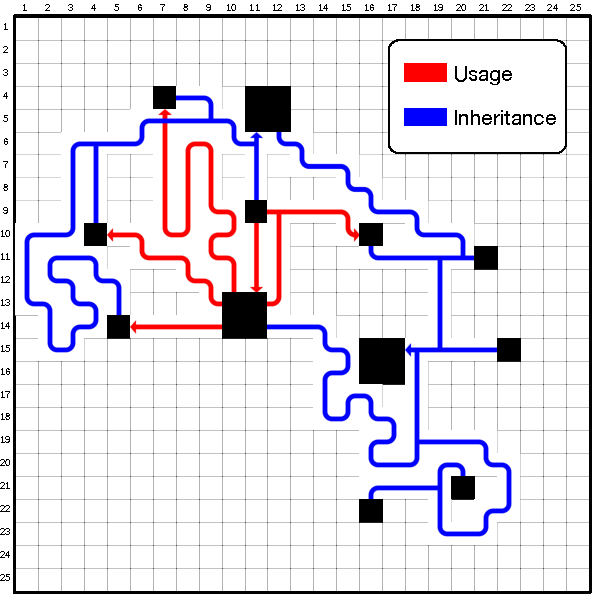
\includegraphics[width=\textwidth]{figures/application/multi_rel_12_classes}
        \caption{\wassis (WFC-pure).}
        \label{fig:multi_rel_pure}
    \end{subfigure}
    \hfill
    \begin{subfigure}[b]{0.48\textwidth}
        \centering
        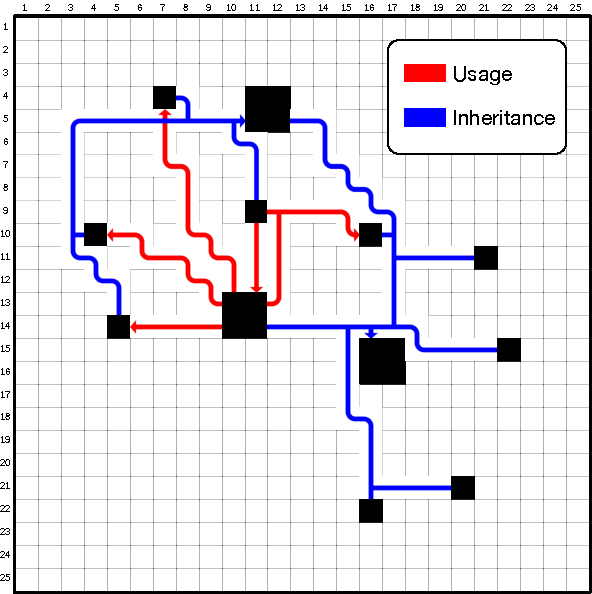
\includegraphics[width=\textwidth]{figures/application/multi_rel_12_classes_opt}
        \caption{\wassis (after path optimization).}
        \label{fig:multi_rel_optimized}
    \end{subfigure}

    \vspace{1em}

    \begin{subfigure}[b]{\textwidth}
        \centering
        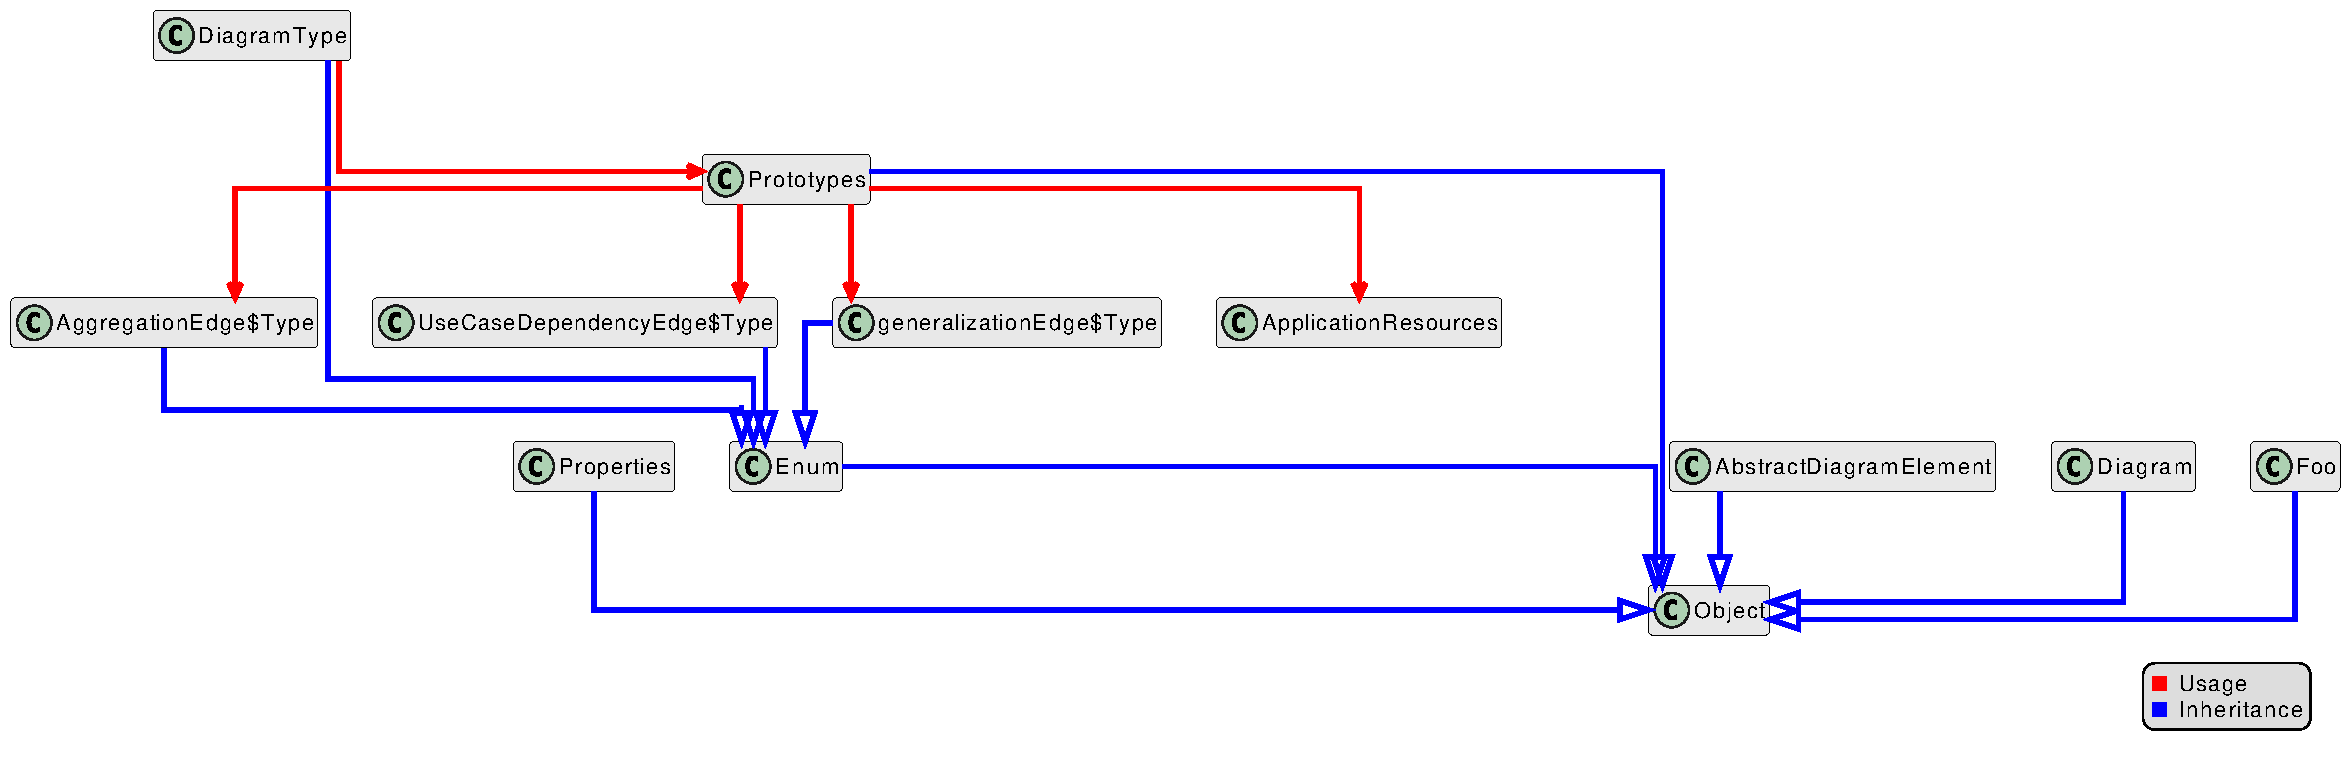
\includegraphics[width=0.97\textwidth]{figures/application/multi_rel_plantuml}
        \caption{\plantuml.}
        \label{fig:multi_rel_plantuml}
    \end{subfigure}

    \caption{Comparison of \wassis and \plantuml for multi-relationship visualization.}
    \label{fig:multi_relationship_comparison}
\end{figure}

\subsection{Path Crossings and Visual Clutter}
Both \wassis and \plantuml have one crossing in this example. In \wassis, the crossing is between a red \texttt{Usage} path and a blue \texttt{Inheritance} path. This crossing is caused by the position of the classes and could have been avoided with a different class placement.

The main difference is the amount of visual clutter. \plantuml draws a separate arrow for each relationship. This creates many lines around classes such as \texttt{Object} and \texttt{Enum}. In \wassis, paths of the same type are merged before reaching the target class. This reduces the overall number of lines in the canvas, making the visualization cleaner.

\subsection{Execution Statistics}
\plantuml generates the layout almost immediately, while \wassis needed more time to find a valid WFC solution on the $25 \times 25$ grid. The execution metrics are shown in \tabref{tab:wassis_multi_rel_stats}.

\begin{table}[ht]
    \centering
    \rowcolors{3}{xcolorblue}{white}
    \begin{tabular}{lr}
        \textbf{Metric} & \textbf{Value} \\ \hline
        Classes & 12 \\
        Paths & 7 \\
        Grid Size & $25 \times 25$ \\
        Path Crossings & 1 \\
        Retries & 11,282 \\
        Execution Time & 17m 15s \\ \hline
    \end{tabular}
    \caption{\wassis execution metrics.}
    \label{tab:wassis_multi_rel_stats}
\end{table}

\wassis found a valid solution after 17 minutes and 15 seconds and 11,282 retries.

\subsection{Summary}
The main differences between \wassis and \plantuml are summarized in \tabref{tab:wassis_plantuml_multi_rel_summary}.

\begin{table}[ht]
    \centering
    \rowcolors{3}{xcolorblue}{white}
    \begin{tabular}{p{0.20\textwidth} p{0.34\textwidth} p{0.34\textwidth}}
        & \textbf{Wassis} & \textbf{PlantUML} \\ 
        
        \hline

        \textbf{Crossings}
        & 1
        & 1 \\

        \textbf{Visual Clutter}
        & Lower, due to path merging.
        & Higher, due to separate arrows. \\

        \textbf{Layout}
        & Star layout.
        & Hierarchical layout. \\

        \textbf{Execution Time}
        & 17m 15s.
        & Milliseconds. \\ 

        \hline
    \end{tabular}
    \caption{Comparison of \wassis and \plantuml.}
    \label{tab:wassis_plantuml_multi_rel_summary}
\end{table}

\end{document}